\subsection{Diagrammi delle classi del ViewModel}
\subsubsection{Package Controllers}
\begin{figure}[h!]
	\begin{center}
		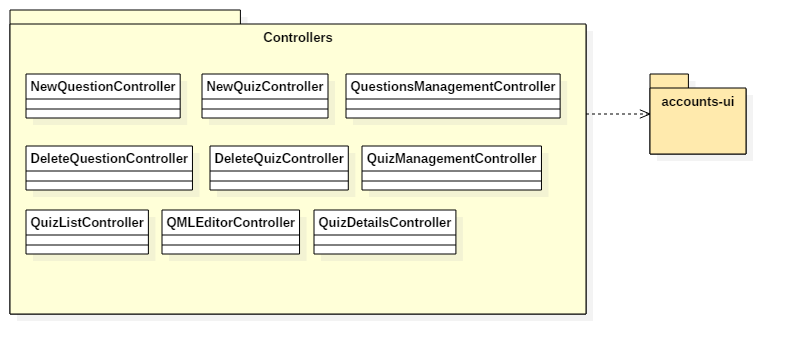
\includegraphics[scale=0.6]{../images/ControllersClass.png}
		\caption{Diagramma delle classi del package Controllers}
	\end{center}
\end{figure}

\subsubsubsection{Classe NewQuestionController}

\begin{itemize}
	\item\textbf{Funzione del componente}: la classe permette di gestire la creazione di una nuova domanda;
	\item\textbf{Relazione d'uso di altre componenti}: il controller è collegato al template. Si relaziona inoltre con  l'editor QML;
	\item\textbf{Attività svolte e dati trattati}: Fornisce le funzionalità per la creazione di una domanda, quali la scelta della categoria e l'inserimento del testo, e espone la funzione di salvataggio dei dati inseriti che compongono la nuova domanda.
\end{itemize}

\subsubsubsection{Classe NewQuizController}

\begin{itemize}
	\item\textbf{Funzione del componente}: la classe permette di gestire la creazione di un nuovo quiz (questionario); 
	\item\textbf{Relazione d'uso di altre componenti}: il controller è collegato al template;
	\item\textbf{Attività svolte e dati trattati}: fornisce le funzionalità per la creazione del nuovo quiz, tramite la scelta di più domande e la scelta della categoria. Espone la funzione di salvataggio del nuovo quiz.
\end{itemize}

\subsubsubsection{Classe QuizListController}

\begin{itemize}
	\item\textbf{Funzione del componente}:  la classe permette il caricamento e la visualizzazione della lista di quiz disponibili nel sistema;
	\item\textbf{Relazione d'uso di altre componenti}: il controller è collegato al templat.; Si relaziona inoltre con il modulo QuizDetails per la visualizzazione dei dettagli di un quiz;
	\item\textbf{Attività svolte e dati trattati}: la classe si occupa di caricare la lista aggiornata dei quiz creati dagli utenti, e fornisce funzionalità di ordinamento della stessa e di selezione dei singoli quiz per la visualizzazione dei dettagli. 
\end{itemize}

\subsubsubsection{Classe QuizDetailsController}

\begin{itemize}
	\item\textbf{Funzione del componente}: la classe permette di visualizzare le informazioni generali di un quiz, una volta selezionato dalla lista dei quiz;
	\item\textbf{Relazione d'uso di altre componenti}: il controller è collegato al template. Si relaziona inoltre con il modulo QuizList.
	\item\textbf{Attività svolte e dati trattati}: la classe si occupa di recuperare e rendere visualizzabili le informazioni relative ad un singolo quiz.
\end{itemize}

\subsubsubsection{Classe DeleteQuestionController}

\begin{itemize}
	\item\textbf{Funzione del componente}: la classe fornisce le funzionalità necessarie alla cancellazione di una domanda precedentemente creata;
	\item\textbf{Relazione d'uso di altre componenti}: il controller è collegato al template. Si relaziona inoltre con il package Methods.
	\item\textbf{Attività svolte e dati trattati}: la classe si occupa di richiedere la cancellazione di una domanda, precedentemente creata dall'utente, dal sistema.
\end{itemize}

\subsubsubsection{Classe DeleteQuizController}

\begin{itemize}
	\item\textbf{Funzione del componente}: la classe fornisce le funzionalità necessarie alla cancellazione di un quiz precedentemente creato;
	\item\textbf{Relazione d'uso di altre componenti}: il controller è collegato al template. Si relaziona inoltre con il package Methods.
	\item\textbf{Attività svolte e dati trattati}:  la classe si occupa di richiedere la cancellazione di un quiz, precedentemente creato dall'utente, dal sistema.
\end{itemize}

\subsubsubsection{Classe QuizManagementController}

\begin{itemize}
	\item\textbf{Funzione del componente}: la classe permette di gestire la somministrazione di un questionario;
	\item\textbf{Relazione d'uso di altre componenti}: il controller è collegato al template. Si relaziona inoltre con il modulo QuestionsManagement;
	\item\textbf{Attività svolte e dati trattati}: la classe si occupa di gestire la risoluzione di un questionario da parte di un utente fornendo la possibilità di navigare tra le domande, salvando le risposte dell'utente e gestendo il tempo limite. Espone la funzione di consegna del quiz compilato.
\end{itemize}

\subsubsubsection{Classe QuestionsManagementController}

\begin{itemize}
	\item\textbf{Funzione del componente}: la classe permette di gestire la somministrazione di una singola domanda all'interno di un questionario;
	\item\textbf{Relazione d'uso di altre componenti}: il controller è collegato al template. Si relaziona inoltre con il modulo QuizManagement;
	\item\textbf{Attività svolte e dati trattati}: la classe si occupa di recuperare i dati associati ad una singola domanda di un questionario e di presentarli all'utente. Tali operazioni si svolgono durante la somministrazione all'utente di un questionario.
\end{itemize}

\subsubsubsection{Classe QMLEditorController}

\begin{itemize}
	\item\textbf{Funzione del componente}: fornisce le funzionalità per creare e modificare una domanda tramite editor QML;
	\item\textbf{Relazione d'uso di altre componenti}: il controller è collegato al template. Si relaziona inoltre con il modulo NewQuestion;
	\item\textbf{Attività svolte e dati trattati}: la classe definisce la logica dello strumento principale di creazione delle domande, l'editor QML, gestisce il testo che viene inserito e espone la funzionalità di checking sintattico del testo inserito.
\end{itemize}

\subsubsubsection{Classe Controller}

\begin{itemize}
	\item\textbf{Funzione del componente}: 
	\item\textbf{Relazione d'uso di altre componenti}: 
	\item\textbf{Attività svolte e dati trattati}:
\end{itemize}

			\subsubsection{Package Subscribers}
\begin{figure}[h!]
\begin{center}
	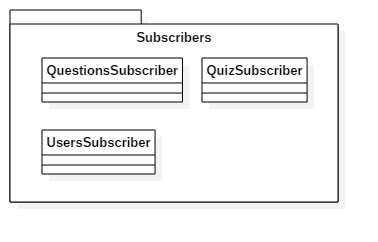
\includegraphics[scale=0.65]{../images/SubscribersClass.png}
	\caption{Diagramma delle classi del package Subscribers}
\end{center}
\end{figure}

\subsubsubsection{Classe QuestionsSubscriber}

\begin{itemize}
	\item\textbf{Funzione del componente}: 
	\item\textbf{Relazione d'uso di altre componenti}: 
	\item\textbf{Attività svolte e dati trattati}:
\end{itemize}

\subsubsubsection{Classe QuizSubscriber}

\begin{itemize}
	\item\textbf{Funzione del componente}: 
	\item\textbf{Relazione d'uso di altre componenti}: 
	\item\textbf{Attività svolte e dati trattati}:
\end{itemize}

\subsubsubsection{Classe UsersSubscriber}

\begin{itemize}
	\item\textbf{Funzione del componente}: 
	\item\textbf{Relazione d'uso di altre componenti}: 
	\item\textbf{Attività svolte e dati trattati}:
\end{itemize}

\subsubsection{Package Methods}
\begin{figure}[h!]
\begin{center}
	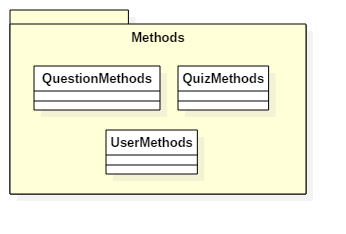
\includegraphics[scale=0.65]{../images/MethodsClass.png}
	\caption{Diagramma delle classi del package Methods}
\end{center}
\end{figure}

\begin{itemize}
	\item\textbf{Funzione del componente}: 
	\item\textbf{Relazione d'uso di altre componenti}: 
	\item\textbf{Attività svolte e dati trattati}:
\end{itemize}

\begin{itemize}
	\item\textbf{Funzione del componente}: 
	\item\textbf{Relazione d'uso di altre componenti}: 
	\item\textbf{Attività svolte e dati trattati}:
\end{itemize}

\begin{itemize}
	\item\textbf{Funzione del componente}: 
	\item\textbf{Relazione d'uso di altre componenti}: 
	\item\textbf{Attività svolte e dati trattati}:
\end{itemize}

\subsubsection{Package QuestionManager}	
Il package fa uso del design pattern \emph{Abstract Factory}.
\begin{figure}[h!]
\begin{center}
	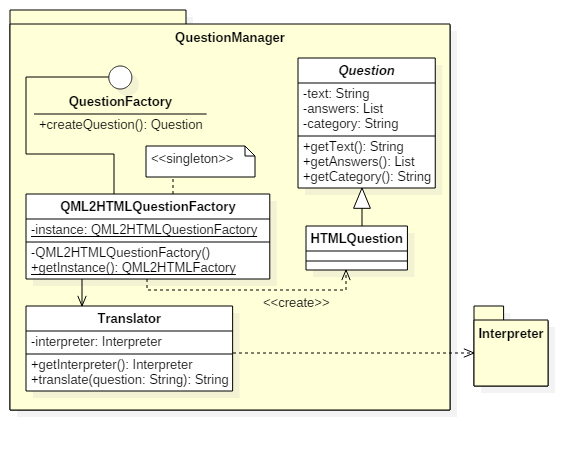
\includegraphics[scale=0.65]{../images/QuestionManagerClass.png}
	\caption{Diagramma delle classi del package QuestionManager}
\end{center}
\end{figure}
\subsubsubsection{Interfaccia QuestionFactory}
\begin{itemize}
	\item\textbf{Funzione del componente}: interfaccia di base delle Factory di tipi Question.
	\item\textbf{Relazione d'uso di altre componenti}: può essere concretizzata in diversi tipi di QuestionFactory.
	\item\textbf{Attività svolte e dati trattati}: definisce il contratto delle factory Question, cioè le operazioni di costruzione di Question che saranno definite in ogni concretizzazione.
\end{itemize}

\subsubsubsection{Classe astratta Question}
\begin{itemize}
	\item\textbf{Funzione del componente}: classe di base del tipo Question.
	\item\textbf{Relazione d'uso di altre componenti}: può essere concretizzata in diversi tipi di Question.
	\item\textbf{Attività svolte e dati trattati}: definisce il contratto generale delle Question, cioè le loro operazioni e dati.
\end{itemize}

\subsubsubsection{Classe QML2HTMLQuestionFactory}
La classe QML2HTMLQuestionFactory è un \emph{singleton}.
\begin{itemize}
	\item\textbf{Funzione del componente}: crea oggetti di tipo HTMLQuestion.
	\item\textbf{Relazione d'uso di altre componenti}: è concretizzazione della classe QuestionFactory. Crea oggetti HTMLQuestion. Si interfaccia con la classe Translator.
	\item\textbf{Attività svolte e dati trattati}: crea su richiesta oggetti di tipo HTMLQuestion, delegando la traduzione del codice QML alla classe Translator.
\end{itemize}

\subsubsubsection{Classe HTMLQuestion}	
\begin{itemize}
	\item\textbf{Funzione del componente}: rappresenta una domanda in formato HTML.
	\item\textbf{Relazione d'uso di altre componenti}: è concretizzazione di Question.
	\item\textbf{Attività svolte e dati trattati}: eredita e specializza le funzionalità dell'interfaccia Question.
\end{itemize}

\subsubsubsection{Classe Translator}
\begin{itemize}
	\item\textbf{Funzione del componente}: s'interfaccia con le componenti del package Interpreter per la traduzione di quesiti QML in HTML.
	\item\textbf{Relazione d'uso di altre componenti}: collabora con le interfacce Interpreter e InterpreterFactory.
	\item\textbf{Attività svolte e dati trattati}: riceve dalla classe ViewUpdater le richieste di traduzione e il codice QML da tradurre. Attraverso la factory InterpreterFactory (una sua concretizzazione) costruisce un Interpreter concreto e lo utilizza per la traduzione del codice. L'esito della traduzione viene reso disponibile a ViewUpdater.
\end{itemize}
\newpage

\subsubsection{Package QuizManager}
Il package fa uso del design pattern \emph{Builder}.
\begin{figure}[h!]
\begin{center}
	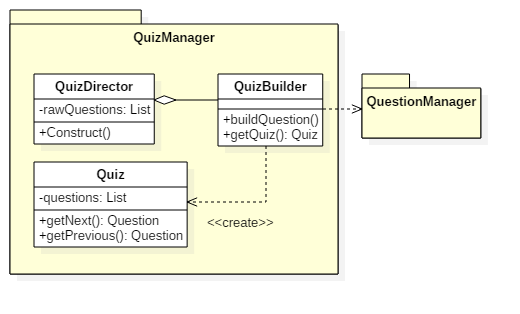
\includegraphics[scale=0.65]{../images/QuizManagerClass.png}
	\caption{Diagramma delle classi del package QuizManager}
\end{center}
\end{figure}
\subsubsubsection{Classe QuizDirector}
\begin{itemize}
\item\textbf{Funzione del componente}: è responsabile della costruzione di un oggetto di tipo Quiz.
	\item\textbf{Relazione d'uso di altre componenti}: utilizza la classe QuizBuilder.
	\item\textbf{Attività svolte e dati trattati}: la classe, a partire da un set di domande (in questo caso in QML), utilizza il Builder per costruire un Quiz.
\end{itemize}

\subsubsubsection{Classe QuizBuilder}
\begin{itemize}
\item\textbf{Funzione del componente}: Costruisce domanda per domanda un questionario.
	\item\textbf{Relazione d'uso di altre componenti}: interagisce con il package QuestionManager.
	\item\textbf{Attività svolte e dati trattati}: Costruisce passo pe r passo un oggetto di tipo Quiz. Si appoggia al package QuestionManager per la creazione delle singole domande.
\end{itemize}

\subsubsubsection{Classe Quiz}
\begin{itemize}
\item\textbf{Funzione del componente}: la classe rappresenta un Quiz, una raccolta di domande.
	\item\textbf{Relazione d'uso di altre componenti}: nessuna.
	\item\textbf{Attività svolte e dati trattati}: la classe possiede i dati e fornisce le operazioni necessaria alla fruizione di un Quiz.
\end{itemize}
\clearpage			

\subsubsection{Package Interpreter}
\begin{figure}[h!]
\begin{center}
	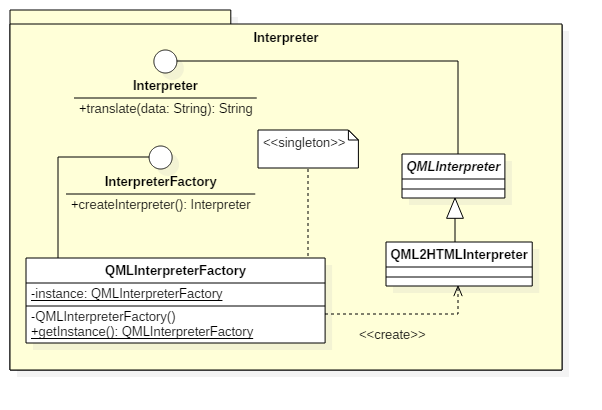
\includegraphics[scale=0.65]{../images/InterpreterClass.png}
	\caption{Diagramma delle classi del package Interpreter}
\end{center}
\end{figure}
\subsubsubsection{Interfaccia Interpreter}
\begin{itemize}
	\item\textbf{Funzione del componente}: interfaccia di base del tipo Interpreter.
	\item\textbf{Relazione d'uso di altre componenti}: può essere concretizzata in diversi tipi di Interpreter. Viene riferita dalla classe Translator.
	\item\textbf{Attività svolte e dati trattati}: definisce il contratto degli Interpreter, cioè le operazioni di traduzione che saranno definite in ogni concretizzazione.
\end{itemize}
\subsubsubsection{Interfaccia InterpreterFactory}
\begin{itemize}
	\item\textbf{Funzione del componente}: interfaccia di base delle Factory di tipi Interpreter.
	\item\textbf{Relazione d'uso di altre componenti}: può essere concretizzata in diversi tipi di InterpreterFactory. Viene riferita dalla classe Translator.
	\item\textbf{Attività svolte e dati trattati}: definisce il contratto delle factory, cioè le operazioni di costruzione di Interpreter che saranno definite in ogni concretizzazione.
\end{itemize}
\subsubsubsection{Classe QMLInterpreterFactory}
La classe QMLInterpreterFactory è un \emph{singleton}.
\begin{itemize}
	\item\textbf{Funzione del componente}: crea oggetti di tipo QMLInterpreter.
	\item\textbf{Relazione d'uso di altre componenti}: è concretizzazione della classe InterpreterFactory. Crea oggetti QMLInterpreter.
	\item\textbf{Attività svolte e dati trattati}: crea su richiesta oggetti di tipo QMLInterpreter.
\end{itemize}
\subsubsubsection{Classe QMLInterpreter}
\begin{itemize}
	\item\textbf{Funzione del componente}: classe astratta che rappresenta gli Interpreter che traducono codice QML in un altro formato.
	\item\textbf{Relazione d'uso di altre componenti}: è sottotipo di Interpreter. Può essere concretizzata in più tipi di QMLInterpreter.
	\item\textbf{Attività svolte e dati trattati}: definisce il contratto dei QMLInterpreter, cioè le operazioni di traduzione da QML verso altri linguaggi.
\end{itemize}
\subsubsubsection{Classe QML2HTMLInterpreter}	
\begin{itemize}
	\item\textbf{Funzione del componente}: traduce codice QML in codice HTML.
	\item\textbf{Relazione d'uso di altre componenti}: è concretizzazione di QMLInterpreter.
	\item\textbf{Attività svolte e dati trattati}: riceve in input domande in QML e le traduce in codice HTML visualizzabile da browser.
\end{itemize}
\newpage